\PassOptionsToPackage{unicode=true}{hyperref} % options for packages loaded elsewhere
\PassOptionsToPackage{hyphens}{url}
%
\documentclass[]{article}
\usepackage[fontset=ubuntu]{ctex}
\usepackage[a4paper,scale=0.8]{geometry}
\usepackage{lmodern}
\usepackage{amssymb,amsmath}
\usepackage{ifxetex,ifluatex}
\usepackage{fixltx2e} % provides \textsubscript
\ifnum 0\ifxetex 1\fi\ifluatex 1\fi=0 % if pdftex
  \usepackage[T1]{fontenc}
  \usepackage[utf8]{inputenc}
  \usepackage{textcomp} % provides euro and other symbols
\else % if luatex or xelatex
  \usepackage{unicode-math}
  \defaultfontfeatures{Ligatures=TeX,Scale=MatchLowercase}
\fi
% use upquote if available, for straight quotes in verbatim environments
\IfFileExists{upquote.sty}{\usepackage{upquote}}{}
% use microtype if available
\IfFileExists{microtype.sty}{%
\usepackage[]{microtype}
\UseMicrotypeSet[protrusion]{basicmath} % disable protrusion for tt fonts
}{}
\IfFileExists{parskip.sty}{%
\usepackage{parskip}
}{% else
\setlength{\parindent}{0pt}
\setlength{\parskip}{6pt plus 2pt minus 1pt}
}
\usepackage{hyperref}
\hypersetup{
            pdfborder={0 0 0},
            breaklinks=true}
\urlstyle{same}  % don't use monospace font for urls
\usepackage{color}
\usepackage{fancyvrb}
\newcommand{\VerbBar}{|}
\newcommand{\VERB}{\Verb[commandchars=\\\{\}]}
\DefineVerbatimEnvironment{Highlighting}{Verbatim}{commandchars=\\\{\}}
% Add ',fontsize=\small' for more characters per line
\newenvironment{Shaded}{}{}
\newcommand{\AlertTok}[1]{\textcolor[rgb]{1.00,0.00,0.00}{\textbf{#1}}}
\newcommand{\AnnotationTok}[1]{\textcolor[rgb]{0.38,0.63,0.69}{\textbf{\textit{#1}}}}
\newcommand{\AttributeTok}[1]{\textcolor[rgb]{0.49,0.56,0.16}{#1}}
\newcommand{\BaseNTok}[1]{\textcolor[rgb]{0.25,0.63,0.44}{#1}}
\newcommand{\BuiltInTok}[1]{#1}
\newcommand{\CharTok}[1]{\textcolor[rgb]{0.25,0.44,0.63}{#1}}
\newcommand{\CommentTok}[1]{\textcolor[rgb]{0.38,0.63,0.69}{\textit{#1}}}
\newcommand{\CommentVarTok}[1]{\textcolor[rgb]{0.38,0.63,0.69}{\textbf{\textit{#1}}}}
\newcommand{\ConstantTok}[1]{\textcolor[rgb]{0.53,0.00,0.00}{#1}}
\newcommand{\ControlFlowTok}[1]{\textcolor[rgb]{0.00,0.44,0.13}{\textbf{#1}}}
\newcommand{\DataTypeTok}[1]{\textcolor[rgb]{0.56,0.13,0.00}{#1}}
\newcommand{\DecValTok}[1]{\textcolor[rgb]{0.25,0.63,0.44}{#1}}
\newcommand{\DocumentationTok}[1]{\textcolor[rgb]{0.73,0.13,0.13}{\textit{#1}}}
\newcommand{\ErrorTok}[1]{\textcolor[rgb]{1.00,0.00,0.00}{\textbf{#1}}}
\newcommand{\ExtensionTok}[1]{#1}
\newcommand{\FloatTok}[1]{\textcolor[rgb]{0.25,0.63,0.44}{#1}}
\newcommand{\FunctionTok}[1]{\textcolor[rgb]{0.02,0.16,0.49}{#1}}
\newcommand{\ImportTok}[1]{#1}
\newcommand{\InformationTok}[1]{\textcolor[rgb]{0.38,0.63,0.69}{\textbf{\textit{#1}}}}
\newcommand{\KeywordTok}[1]{\textcolor[rgb]{0.00,0.44,0.13}{\textbf{#1}}}
\newcommand{\NormalTok}[1]{#1}
\newcommand{\OperatorTok}[1]{\textcolor[rgb]{0.40,0.40,0.40}{#1}}
\newcommand{\OtherTok}[1]{\textcolor[rgb]{0.00,0.44,0.13}{#1}}
\newcommand{\PreprocessorTok}[1]{\textcolor[rgb]{0.74,0.48,0.00}{#1}}
\newcommand{\RegionMarkerTok}[1]{#1}
\newcommand{\SpecialCharTok}[1]{\textcolor[rgb]{0.25,0.44,0.63}{#1}}
\newcommand{\SpecialStringTok}[1]{\textcolor[rgb]{0.73,0.40,0.53}{#1}}
\newcommand{\StringTok}[1]{\textcolor[rgb]{0.25,0.44,0.63}{#1}}
\newcommand{\VariableTok}[1]{\textcolor[rgb]{0.10,0.09,0.49}{#1}}
\newcommand{\VerbatimStringTok}[1]{\textcolor[rgb]{0.25,0.44,0.63}{#1}}
\newcommand{\WarningTok}[1]{\textcolor[rgb]{0.38,0.63,0.69}{\textbf{\textit{#1}}}}
\usepackage{graphicx,grffile}
\makeatletter
\def\maxwidth{\ifdim\Gin@nat@width>\linewidth\linewidth\else\Gin@nat@width\fi}
\def\maxheight{\ifdim\Gin@nat@height>\textheight\textheight\else\Gin@nat@height\fi}
\makeatother
% Scale images if necessary, so that they will not overflow the page
% margins by default, and it is still possible to overwrite the defaults
% using explicit options in \includegraphics[width, height, ...]{}
\setkeys{Gin}{width=\maxwidth,height=\maxheight,keepaspectratio}
\setlength{\emergencystretch}{3em}  % prevent overfull lines
\providecommand{\tightlist}{%
  \setlength{\itemsep}{0pt}\setlength{\parskip}{0pt}}
\setcounter{secnumdepth}{0}
% Redefines (sub)paragraphs to behave more like sections
\ifx\paragraph\undefined\else
\let\oldparagraph\paragraph
\renewcommand{\paragraph}[1]{\oldparagraph{#1}\mbox{}}
\fi
\ifx\subparagraph\undefined\else
\let\oldsubparagraph\subparagraph
\renewcommand{\subparagraph}[1]{\oldsubparagraph{#1}\mbox{}}
\fi

% set default figure placement to htbp
\makeatletter
\def\fps@figure{htbp}
\makeatother

\title{第一次作业}
\author{BobAnkh}
\date{}

\begin{document}

\maketitle

\hypertarget{header-n1}{%
\subsection{1. 结合日常生活中的感受,归纳视觉与听觉信息的产生、传播、获取的特点。}\label{header-n1}}

视觉信息,也就是图像信息,是基于光这种物质产生,经由光学、化学和神经处理等过程得到的;它可以通过图像媒体(照片,胶片,数字存储体等)传递、共享;它由人类视觉系统感知获取

听觉信息,也就是声音信息,是基于声波这种物质产生,由物体振动产生的机械波得到;它通过介质传播,通过声音记录媒体(磁带,唱片,
CD 等)传递、共享;它由人的听觉系统感知获取

\hypertarget{header-n2}{%
\subsection{2. 工作波长为510nm的激光器,其发光的辐射通量为1瓦特,分别求其在明视觉以及暗视觉下的光通量。(510nm波长光的光谱光效率函数值为0.503(明视觉),0.997(暗视觉,注意暗视觉下光通量定义有变化))。}\label{header-n2}}

明视觉:\(\Phi_v=683\times\Phi_e(\lambda)\times V(\lambda)=683\times 1\times 0.503=343.549(lm)\)

暗视觉:\(\Phi_v=1699\times\Phi_e(\lambda)\times V(\lambda)=683\times 1\times 0.997=1693.903(lm)\)

\hypertarget{header-n80}{%
\subsection{3. CIE物理三基色R,G,B的光谱光效率函数值分别为0.0041, 0.9756, 0.0173,如果R光通量为1lm, G光通量为4.5907lm, B光通量为0.0601lm可以合成白光,计算该白光的光通量和辐射通量现。}\label{header-n80}}

该白光的光通量为:\(\Phi_v=1+4.5907+0.0601=5.6508(lm)\)

要计算白光的辐射通量,则应当计算各分光的辐射通量,然后加起来:

R:
\(\Phi_e=\frac{\Phi_v}{683\times V(\lambda)}=\frac{1}{683\times 0.0041}=0.3571(W)\)

G:
\(\Phi_e=\frac{\Phi_v}{683\times V(\lambda)}=\frac{4.5907}{683\times 0.9756}=0.0069(W)\)

B:
\(\Phi_e=\frac{\Phi_v}{683\times V(\lambda)}=\frac{0.0601}{683\times 0.0173}=0.0051(W)\)

由此得到白光的辐射功率:\(\Phi_e=0.3571+0.0069+0.0051=0.3691(W)\)

\hypertarget{header-n4}{%
\subsection{4. 在一个没有遮挡的空地上水平放置一块边长为0.5米的方形平板,在一个多云天气,天空的辐射亮度均匀为$1000W/m^2∙sr$,试计算平板中心点的辐射照度;如果平板是一个理想漫反射表面且漫反射系数$k_d=0.4$,试计算平板中心处法向量方向,以及和法向量夹角为$45^°$方向上的反射辐射亮度。}\label{header-n4}}

平板中心点辐射照度:\(E=\int_{\Omega}L(\omega)cos\theta d\omega=\pi L=1000\pi (W/m^2)\)

若平板是理想漫反射表面,则反射幅度亮度与观察角度无关,即平板中心法向量方向和与法向量夹角\(45^\circ\)方向上的反射辐射亮度是一样的,均可通过下式求得:

\(L_e=\int_{\Omega}\rho L(\omega_i)cos\theta_i d\omega_i=\rho E_i=\frac{k_d}{\pi}E_i=\frac{0.4}{\pi}1000\pi=400(W/m^2\cdot sr)\)

\hypertarget{header-n80}{%
\subsection{5. 某彩色光由物理三基色混配出,其中红基色光10lm,绿基色光23lm,蓝基色光3lm,求该彩色光在CIE-RGB和CIE-XYZ中的配色方程以及色度坐标。}\label{header-n80}}

CIE-RGB:

色系数: \(R=10/1=10,G=23/4.5907=5,B=3/0.0601=50\)

配色方程为: \(10[R]+5[G]+50[B]\)

色度坐标为:
\((r,g,b)=(\frac{R}{R+G+B},\frac{G}{R+G+B},\frac{B}{R+G+B})=(\frac{10}{65},\frac{5}{65},\frac{50}{65})=(0.1538,0.0769,0.7692)\)

CIE-XYZ:

色系数:
\(\begin{bmatrix}X \\Y \\ Z\end{bmatrix}=\begin{bmatrix}2.7689 & 1.7518 & 1.1302 \\1.0000 & 4.5907 & 0.0601 \\ 0.0000 & 0.0565 & 5.5943 \end{bmatrix}\begin{bmatrix}R \\ G \\ B\end{bmatrix}\)

可以算出:
\(\begin{bmatrix}X \\ Y \\ Z\end{bmatrix}=\begin{bmatrix}93 \\ 36 \\ 280 \end{bmatrix}\)

配色方程为: \(93[X]+36[Y]+280[Z]\)

色度坐标为:
\((x,y,Y)=(\frac{X}{X+Y+Z},\frac{Y}{X+Y+Z},Y)=(\frac{93}{409},\frac{36}{409},36)=(0.2274,0.0880,36)\)

\hypertarget{header-n5}{%
\subsection{6. 已知某色光在CIE-XYZ表色系中的色度坐标为(0.45, 0.15, 15),求该色光的色系数; 求可以和该色光混配出60流明等能白光的补色光配色方程和色度坐标。}\label{header-n5}}

由题意可得色度坐标为: \((x,y,Y)=(0.45,0.15,15)\)

则由此可以求得该色光的各个色系数:
\(X=\frac{Y}{y}x=45,Y=15,Z=\frac{Y}{y}-X-Y=40\)

若设补色光的配色方程为:
\(X_1[X]+Y_1[Y]+Z_1[Z]\),则可以得到混配光的配色方程:
\((45+X_1)[X]+(15+Y_1)[Y]+(40+Z_1)[Z]\)

因为是要混配出60流明等能白光,故应该有:

\(45+X_1=15+Y_1=40+Z_1=60\)

则可以解得: \(X_1=15,Y_1=45,Z_1=20\)

由此得到补色光的配色方程: \(15[X]+45[Y]+20[Z]\)

由此可以计算其色度坐标:
\((x,y,Y)=(\frac{X}{X+Y+Z},\frac{Y}{X+Y+Z},Y)=(\frac{15}{80},\frac{45}{80},45)=(0.1875,0.5625,45)\)

\hypertarget{header-n7}{%
\subsection{7. 用几何的方式证明,在小孔成像中,空间中共面P的两条平行线的投影汇聚到直线H上。H是通过小孔且平行于P的平面与成像面的交线。}\label{header-n7}}

\begin{figure}
\centerline{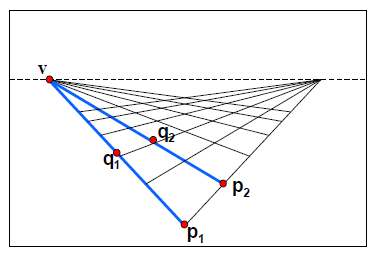
\includegraphics[width=\linewidth]{figures/1-7-ans.png}}
\caption{}
\end{figure}

采用课件上的图片用以说明。取空间中共面\(P\)的两条平行线\(q_1p_1\)和\(q_2p_2\),根据灭点的性质,可以知道它们有共同的灭点\(v\),并且过该灭点和小孔的直线会与\(q_1p_1\)和\(q_2p_2\)平行,这也就意味着这条直线和平面\(P\)平行,则由此过该直线做一个平行于\(P\)的平面\(Q\),那么可知\(v\)必然在该平面与成像面的交线\(H\)上。同理对于另外任意两条在平面\(P\)上的平行线,其共同的灭点也应该位于平面\(Q\)和成像平面上,也就是交线\(H\)上。从而无数多组这样的两条平行线投影汇聚而成就是直线\(H\),同时直线\(H\)是通过小孔且平行于平面\(P\)的平面与成像面的交线。

\hypertarget{header-n8}{%
\subsection{8. 第三章讲义中P45页中,地面的灭线为图像最上方的白线,已知图中男士的身高为1.90米,请估算图中女士的身高。}\label{header-n8}}

\begin{figure}
\centerline{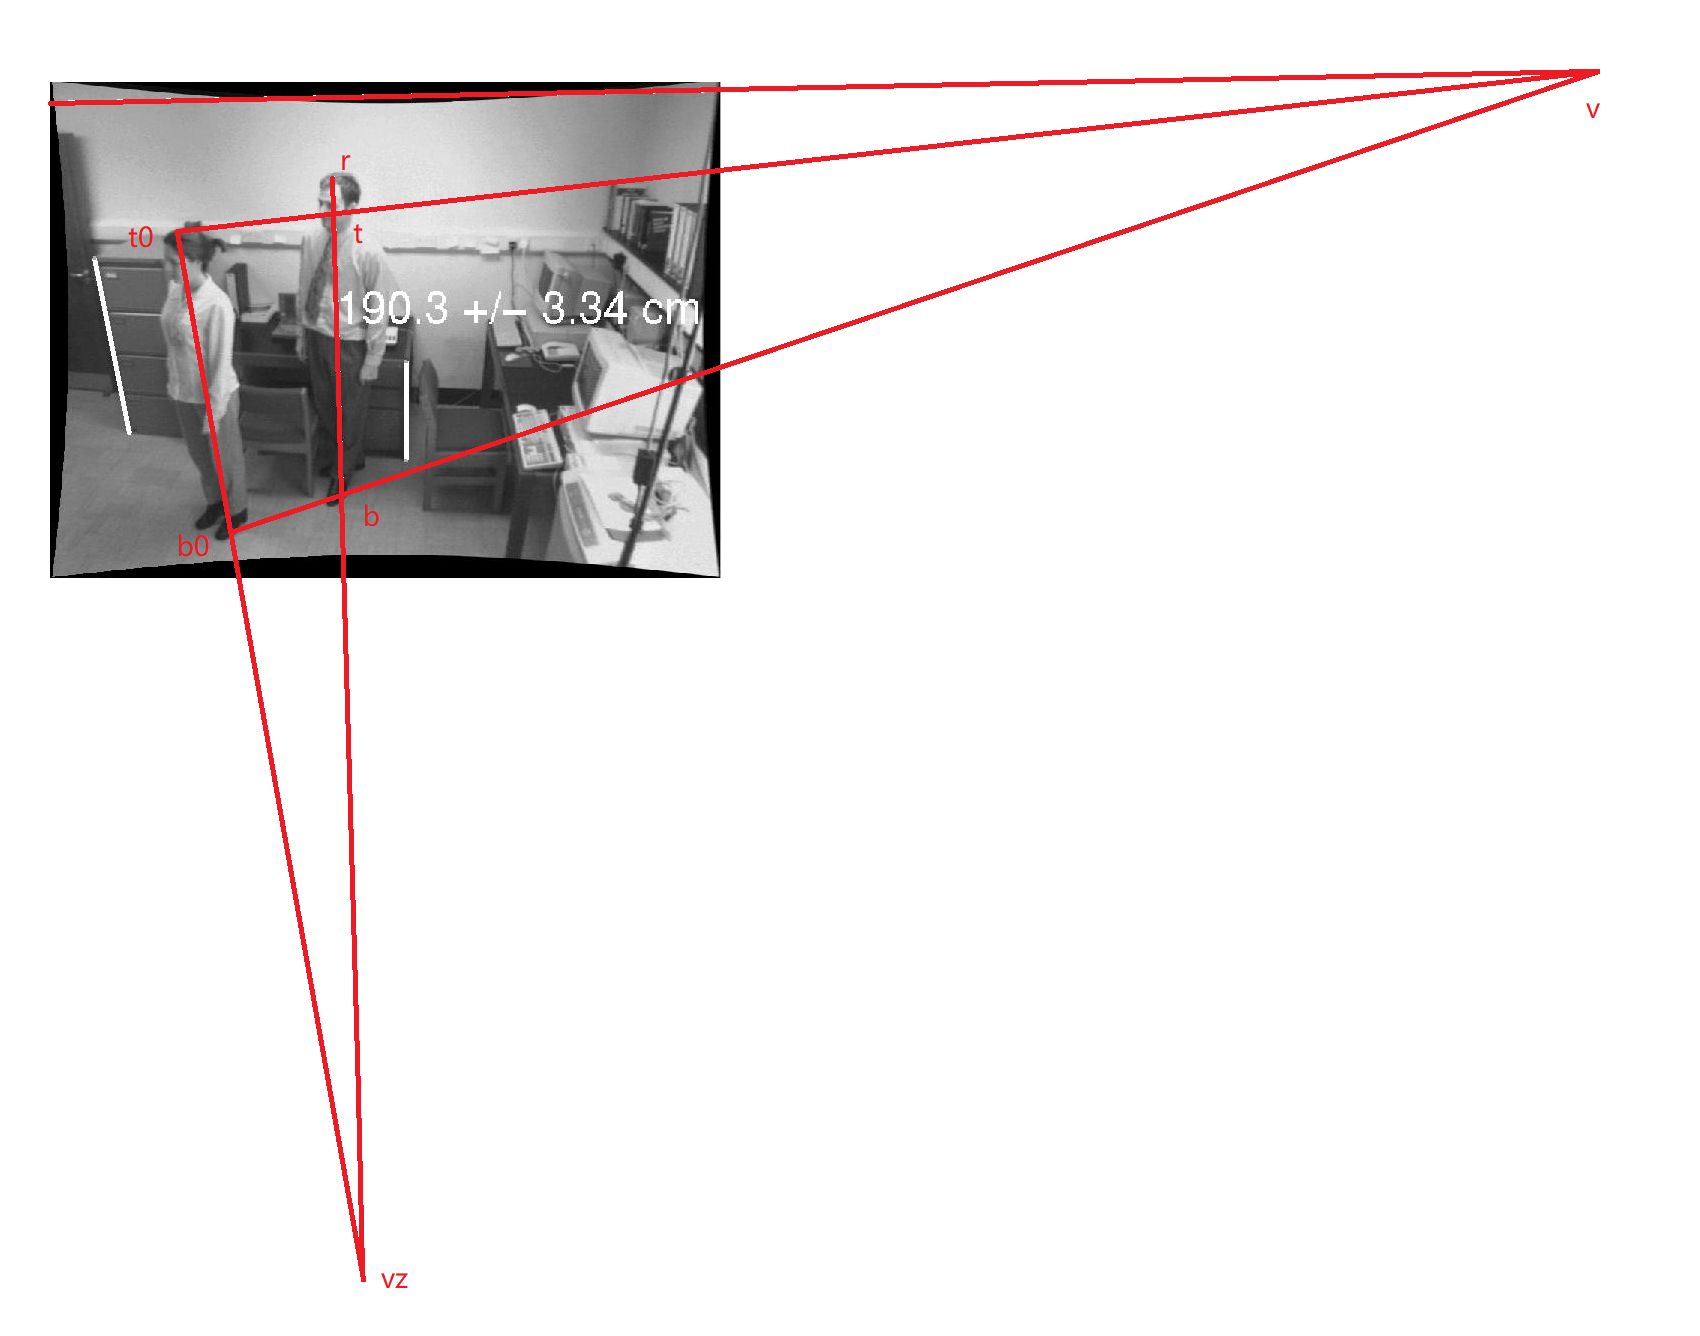
\includegraphics[width=.8\linewidth]{figures/1-8-ans.png}}
\caption{}
\end{figure}

延长灭线,通过绘制各线找到垂直方向的灭点和参考物体的顶点\(r\)和底点\(b\),确定待测物体的顶点\(t_0\)和底点\(b_0\),\(bb_0\)交灭线于灭点\(v\),由此可以确定参考物体上的点\(t\),则根据交比有:
$$
\frac{\lVert t-b\rVert \lVert v_z-r\rVert}{\lVert r-b\rVert\lVert v_z-t\rVert}=\frac{H}{R}
$$

则由此可以估算图中女士的身高:
$$
H=\frac{\lVert t-b\rVert \lVert v_z-r\rVert}{\lVert r-b\rVert\lVert v_z-t\rVert}R=\frac{281.11\times 1099.44}{317.13\times 1063.42}\times 1.90\approx 1.74m
$$

\hypertarget{header-n9}{%
\subsection{9. 相机校准:现要校准一个双目成像系统,由C1、C2两台相机组成,成像分辨率均为640x480像素(宽x高)。以下数据均以Matlab格式给出。}\label{header-n9}}

\textbf{1) 已知:在以C1的成像中心为原点的坐标系下,场景中6个标志点的坐标如下。矩阵中每一列表示一个标志点的三维坐标$(x_s,y_s,z_s)^T$。}
$$
\begin{bmatrix} -319.0 & -183.5 & 81.04 & -40.58 & -183.7 & -48.47 \\
   5.635 & -153.3  & 10.14 &  205.9 & -34.94 &  54.10\\
   585.0 &  603.0 &  615.0 &  599.2 & 591.1  &  610.9\\
\end{bmatrix}
$$

\textbf{这些标志点在C1的照片中的坐标依次如下。矩阵每一列表示一个二维坐标$(x_{pixel},y_{pixel})^T$}
$$
\begin{bmatrix} 78 &  200 &  432 &  325  & 198 &  318\\
257 &  116  & 261  & 432  & 221 &  300\\
\end{bmatrix}
$$

\textbf{数字图像中的坐标系一般规定为下图3所示,且实际只在整数坐标点上存在采样值。}

\begin{figure}
\centerline{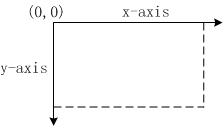
\includegraphics[width=.3\linewidth]{figures/q9.png}}
\caption{}
\end{figure}

\textbf{求:C1的内参数$α_x,α_y,x_0,y_0$(假定skew parameter为0)。}

\textbf{2) 已知:相机C2相对于C1的旋转矩阵R0和平移矢量T0分别为}
$$
R0 = \begin{bmatrix} 0.9998 &  -0.0178 &  -0.0004\\
0.0178   & 0.9998  & -0.0048\\
0.0004   & 0.0048  &  1.0000\\
\end{bmatrix}
$$
$$
T0 = \begin{bmatrix}97.27 & 2.05 & 3.53\end{bmatrix}.';
$$

\textbf{又已知C2的内参数为:}
$$
α_x=546.4,α_y=547.8,x_0=319,y_0=243
$$

\textbf{求:(1)中的标志点在C2的照片中的坐标。注意结果要按(1)中的样式给出。}

\begin{enumerate}
    \item 

相机成像的坐标变换有如下关系:
$$
\begin{bmatrix}u^{'} \\ v^{'} \\ w^{'}\end{bmatrix}=\begin{bmatrix}a_x & 0 & x_0 & 0 \\ 0 & a_y & y_0 & 0 \\ 0 & 0 & 1 & 0 \end{bmatrix} \begin{bmatrix}x_s\\y_s\\z_s\\1\end{bmatrix}\
$$
$$
x_{pix}=\frac{u^{'}}{w^{'}} \\ y_{pix}=\frac{v^{'}}{w^{'}}
$$

一共有6组数据,所以可以得到线性方程组:
$$
\begin{bmatrix}x_{pix1}z_{s1} & \cdots & x_{pix6}z_{s6} \\ y_{pix1}z_{s1} & \cdots & y_{pix6}z_{s6} \\ z_{s1} & \cdots & z_{s6}\end{bmatrix}=\begin{bmatrix}a_x & 0 & x_0 & 0 \\ 0 & a_y & y_0 & 0 \\ 0 & 0 & 1 & 0 \end{bmatrix} \begin{bmatrix}x_{s1} & \cdots & x_{s6}\\y_{s1} & \cdots & y_{s6}\\z_{s1} & \cdots & z_{s6}\\1 & \cdots & 1\end{bmatrix}
$$

整理化简可以得到:
$$
\begin{bmatrix}x_{pix1} \\ y_{pix1} \\ \vdots \\ x_{pix6} \\ y_{pix6} \end{bmatrix}=\begin{bmatrix}\frac{x_{s1}}{z_{s1}} & 0 & 1 & 0 \\ 0 & \frac{y_{s1}}{z_{s1}} & 0 & 1 \\ \vdots & \vdots & \vdots & \vdots \\ \frac{x_{s6}}{z_{s6}} & 0 & 1 & 0 \\ 0 & \frac{y_{s6}}{z_{s6}} & 0 & 1\end{bmatrix}\begin{bmatrix}a_x \\ a_y \\ x_0 \\ y_0\end{bmatrix}
$$

为了方便书写,做如下标记:
$$
X = \begin{bmatrix}x_{pix1} \\ y_{pix1} \\ \vdots \\ x_{pix6} \\ y_{pix6} \end{bmatrix},\,A=\begin{bmatrix}\frac{x_{s1}}{z_{s1}} & 0 & 1 & 0 \\ 0 & \frac{y_{s1}}{z_{s1}} & 0 & 1 \\ \vdots & \vdots & \vdots & \vdots \\ \frac{x_{s6}}{z_{s6}} & 0 & 1 & 0 \\ 0 & \frac{y_{s6}}{z_{s6}} & 0 & 1\end{bmatrix},\,\lambda=\begin{bmatrix}a_x \\ a_y \\ x_0 \\ y_0\end{bmatrix}
$$

则可采用最小二乘法得到结果(使用MATLAB编程辅助计算):
$$
\lambda=\begin{bmatrix}a_x \\ a_y \\ x_0 \\ y_0\end{bmatrix}=(A^TA)^{-1}A^TX=\begin{bmatrix}522.7202\\ 528.4993 \\ 360.9253 \\ 251.7311\end{bmatrix}
$$

MATLAB辅助计算的代码如下:

\begin{Shaded}
\begin{Highlighting}[]
\NormalTok{xsyszs = [-}\FloatTok{319.0}\NormalTok{ -}\FloatTok{183.5}   \FloatTok{81.04}\NormalTok{  -}\FloatTok{40.58}\NormalTok{ -}\FloatTok{183.7}\NormalTok{  -}\FloatTok{48.47}\NormalTok{; ...
}
   \FloatTok{5.635}\NormalTok{ -}\FloatTok{153.3}   \FloatTok{10.14}  \FloatTok{205.9}\NormalTok{  -}\FloatTok{34.94}   \FloatTok{54.10}\NormalTok{; ...
}
   \FloatTok{585.0}  \FloatTok{603.0}   \FloatTok{615.0}  \FloatTok{599.2}  \FloatTok{591.1}    \FloatTok{610.9}\NormalTok{];
}
\NormalTok{xpyp = [}\FloatTok{78}   \FloatTok{200}   \FloatTok{432}   \FloatTok{325}   \FloatTok{198}   \FloatTok{318}\NormalTok{; ...
}
\FloatTok{257}   \FloatTok{116}   \FloatTok{261}   \FloatTok{432}   \FloatTok{221}   \FloatTok{300}\NormalTok{];
}
\NormalTok{X = reshape(xpyp, [], }\FloatTok{1}\NormalTok{);
}
\NormalTok{A = zeros(}\FloatTok{12}\NormalTok{, }\FloatTok{4}\NormalTok{);
}
\NormalTok{for k = }\FloatTok{1}\NormalTok{:}\FloatTok{6}

\NormalTok{    A(}\FloatTok{2}\NormalTok{ * k - }\FloatTok{1}\NormalTok{, }\FloatTok{1}\NormalTok{) = xsyszs(}\FloatTok{1}\NormalTok{, k) / xsyszs(}\FloatTok{3}\NormalTok{, k);
}
\NormalTok{    A(}\FloatTok{2}\NormalTok{ * k - }\FloatTok{1}\NormalTok{, }\FloatTok{3}\NormalTok{) = }\FloatTok{1}\NormalTok{;
}
\NormalTok{    A(}\FloatTok{2}\NormalTok{ * k, }\FloatTok{2}\NormalTok{) = xsyszs(}\FloatTok{2}\NormalTok{, k) / xsyszs(}\FloatTok{3}\NormalTok{, k);
}
\NormalTok{    A(}\FloatTok{2}\NormalTok{ * k, }\FloatTok{4}\NormalTok{) = }\FloatTok{1}\NormalTok{;
}
\NormalTok{end
}
\NormalTok{lambda = (A.' * A)^(-}\FloatTok{1}\NormalTok{) * A.' * X;
}
\NormalTok{disp(lambda);}
\end{Highlighting}
\end{Shaded}

\item

将\(C2\)视作世界坐标系,\(C1\)视作相机坐标系,则有:
$$
\begin{bmatrix} x_s^{(C1)} \\ y_s^{(C1)} \\ z_S^{(C1)} \\ 1\end{bmatrix} = \begin{bmatrix}R & T \\ 0_3^T & 1 \end{bmatrix}\begin{bmatrix}x_s^{(C2)} \\ y_s^{(C2)} \\ z_S^{(C2)} \\ 1\end{bmatrix}
$$

由此可以计算:
$$
\begin{bmatrix}u^{(C2)} \\ v^{(C2)} \\ w^{(C2)}\end{bmatrix}=\begin{bmatrix}a_x & 0 & x_0 & 0 \\ 0 & a_y & y_0 & 0 \\ 0 & 0 & 1 & 0 \end{bmatrix} \begin{bmatrix}x_s^{(C2)} \\ y_s^{(C2)} \\ z_S^{(C2)} \\ 1\end{bmatrix}=\begin{bmatrix}a_x & 0 & x_0 & 0 \\ 0 & a_y & y_0 & 0 \\ 0 & 0 & 1 & 0 \end{bmatrix}\begin{bmatrix}R & T \\ 0_3^T & 1 \end{bmatrix}^{-1}\begin{bmatrix} x_s^{(C1)} \\ y_s^{(C1)} \\ z_S^{(C1)} \\ 1\end{bmatrix}
$$

由此可以计算出在\(C2\)的照片中的坐标:
$$
\begin{bmatrix}x_{pix}^{(C2)} \\ y_{pix}^{(C2)}\end{bmatrix}=\begin{bmatrix}\frac{u^{(C2)}}{w^{(C2)}} \\ \frac{v^{(C2)}}{w^{(C2)}} \end{bmatrix}
$$

使用MATLAB编程辅助计算可以得到结果:
$$
\begin{matrix}[-72 & 61& 305 & 196 & 58 & 189;\,... \\ 256 & 108 & 253 & 436 & 216 & 295] \end{matrix}
$$

MATLAB辅助计算的代码如下:

\begin{Shaded}
\begin{Highlighting}[]
\NormalTok{xsyszs = [-}\FloatTok{319.0}\NormalTok{ -}\FloatTok{183.5}   \FloatTok{81.04}\NormalTok{  -}\FloatTok{40.58}\NormalTok{ -}\FloatTok{183.7}\NormalTok{  -}\FloatTok{48.47}\NormalTok{; ...}
   \FloatTok{5.635}\NormalTok{ -}\FloatTok{153.3}   \FloatTok{10.14}  \FloatTok{205.9}\NormalTok{  -}\FloatTok{34.94}   \FloatTok{54.10}\NormalTok{; ...}
   \FloatTok{585.0}  \FloatTok{603.0}   \FloatTok{615.0}  \FloatTok{599.2}  \FloatTok{591.1}    \FloatTok{610.9}\NormalTok{];}
\NormalTok{R0 = ...}
\NormalTok{   [}\FloatTok{0.9998}\NormalTok{   -}\FloatTok{0.0178}\NormalTok{   -}\FloatTok{0.0004}\NormalTok{; ...}
    \FloatTok{0.0178}    \FloatTok{0.9998}\NormalTok{   -}\FloatTok{0.0048}\NormalTok{; ...}
    \FloatTok{0.0004}    \FloatTok{0.0048}    \FloatTok{1.0000}\NormalTok{];}
\NormalTok{T0 = [}\FloatTok{97.27} \FloatTok{2.05} \FloatTok{3.53}\NormalTok{].';}
\NormalTok{ax = }\FloatTok{546.4}\NormalTok{;}
\NormalTok{ay = }\FloatTok{547.8}\NormalTok{;}
\NormalTok{x0 = }\FloatTok{319}\NormalTok{;}
\NormalTok{y0 = }\FloatTok{243}\NormalTok{;}
\NormalTok{alpha = [ax }\FloatTok{0}\NormalTok{  x0 }\FloatTok{0}\NormalTok{;...}
         \FloatTok{0}\NormalTok{  ay y0 }\FloatTok{0}\NormalTok{;...}
         \FloatTok{0}  \FloatTok{0}  \FloatTok{1}  \FloatTok{0}\NormalTok{;];}
\NormalTok{CT = zeros(}\FloatTok{4}\NormalTok{, }\FloatTok{4}\NormalTok{);}
\NormalTok{CT(}\FloatTok{1}\NormalTok{:}\FloatTok{3}\NormalTok{, }\FloatTok{1}\NormalTok{:}\FloatTok{3}\NormalTok{) = R0;}
\NormalTok{CT(}\FloatTok{1}\NormalTok{:}\FloatTok{3}\NormalTok{, }\FloatTok{4}\NormalTok{) = T0;}
\NormalTok{CT(}\FloatTok{4}\NormalTok{, }\FloatTok{4}\NormalTok{) = }\FloatTok{1}\NormalTok{;}
\NormalTok{xpyp = zeros(}\FloatTok{2}\NormalTok{, }\FloatTok{6}\NormalTok{);}
\NormalTok{for k = }\FloatTok{1}\NormalTok{:}\FloatTok{6}
\NormalTok{    uvw = alpha * CT^(-}\FloatTok{1}\NormalTok{) * [xsyszs(:, k);}\FloatTok{1}\NormalTok{];}
\NormalTok{    xpyp(}\FloatTok{1}\NormalTok{, k) = round(uvw(}\FloatTok{1}\NormalTok{) / uvw(}\FloatTok{3}\NormalTok{));}
\NormalTok{    xpyp(}\FloatTok{2}\NormalTok{, k) = round(uvw(}\FloatTok{2}\NormalTok{) / uvw(}\FloatTok{3}\NormalTok{));}
\NormalTok{end}
\NormalTok{disp(xpyp);}
\end{Highlighting}
\end{Shaded}

\end{enumerate}
\end{document}
